\documentclass[conference]{IEEEtran}
\usepackage{cite}
\usepackage[utf8]{inputenc}
\usepackage{amsmath,amssymb,amsfonts}
\usepackage{algorithm}
\usepackage{algorithmic}
\usepackage{listings}
\usepackage{graphicx}
\usepackage{forest}
\usepackage{textcomp}
\usepackage{ragged2e}
\usepackage{tikz}
\usepackage{hyperref}
\usepackage{appendix}
\usetikzlibrary{automata,positioning}
\graphicspath{ {./images/} }
\def\BibTeX{{\rm B\kern-.05em{\sc i\kern-.025em b}\kern-.08em
    T\kern-.1667em\lower.7ex\hbox{E}\kern-.125emX}}

\title{Proyecto del curso Análisis y Diseño de Algoritmos}

\author{
	\IEEEauthorblockN{1\textsuperscript{st} Piero Morales Alcalde}
	\IEEEauthorblockA{
		\textit{Computer Science Student} \\
		\textit{Universidad de Ingeniería y Tecnología}\\
		Lima, Perú \\
		piero.morales@utec.edu.pe
	}
	\and
	\IEEEauthorblockN{2\textsuperscript{nd} André Segovia Melgarejo}
	\IEEEauthorblockA{
		\textit{Computer Science Student} \\
		\textit{Universidad de Ingeniería y Tecnología}\\
		Lima, Perú \\
		andre.segovia@utec.edu.pe
	}
	\and                                                                                                                                                              
	\IEEEauthorblockN{3\textsuperscript{rd} Osman Vilchez Aguirre}
	\IEEEauthorblockA{
		\textit{Computer Science Student} \\
		\textit{Universidad de Ingeniería y Tecnología}\\
		Lima, Perú \\
		osman.vilchez@utec.edu.pe
	}
}

\begin{document}

\maketitle

\section{Introduction}
En este proyecto se va resolver el problema de \textsc{Min-Matching} con el uso de algoritmos de tipo Greedy y con Programación dinámica.

\section{Problema de Min-Matching}

Dados dos vectores $A$ y $B$ de ceros y unos, se debe encontar un \textbf{matching de peso mínimo}. En cada uno de los vectores se pueden encontrar bloques. Un \textit{bloque} es un subarreglo de unos. Cada bloque puede ser denotado por un par ordenado $[i,j]$, donde $i$ es el índice inicial del bloque y $j$ es el índice final del bloque. Por ejemplo, si $A$ tiene $m$ bloques, entonces se pueden ordenar dichos bloques de forma creciente por índice inicial.\\\\
Ahora, se quiere asociar los segmentos de $A$ con los segmentos de $B$. Más formalmente, un \textit{matching} entre $A$ y $B$ es un conjunto $M$ de pares ordenados $(i,j)$ que comple las siguientes condiciones.\\
\begin{enumerate}
    \item Todo índice entre $1$ y $m$ aparece alguna vez en la primera coordenada de algún par ordenado en $M$. Todo índice entre $1$ y $n$ aparece alguna vez en la segunda coordenada de algún par ordenado en $M$.\\
    \item Si $(i_1,j_2) \in M$, $i_1<i_2$ y $j1<j2$, entonces $(i_2,j_1) \notin M$.\\
    \item Si $(i_1,j_1)$, $(i_2,j_2) \in M$ con $i_1<i_2$ y $j_1<j_2$, entonces $(i_1,j_2)$, $(i_2,j_1) \notin M$.\\
\end{enumerate}
Es decir, un \textit{matching} corresponde a una transformación entre bloques de $A$ hacia los bloques de $B$, tal que algunos bloques de $A$ son divididos y otros bloques son agrupados.\\\\
Formalmente, dado un \textit{matching} entre dos vectores, $A$ y un índice $i$, una i-división es un subconjunto $(i,j_1),(i,j_2),...,(i,j_k)$ del matching original. Note que, debido a la definición de matching, $j_1,j_2,...,j_k$ son índices consecutivos. Y dado un índice $j$, un j-agrupamiento es un subconjunto $(i_1,j),(i_2,j),...,(i_l,j)$ del matching original. Note que, debido a la definición de matching, $i_1,i_2,...,i_l$ son índices consecutivos.\\\\
Si $D=\{(i,j_1),(i,j_2),...,(i,j_k)\}$ es una división, entonces el peso asociado a dicha división es el siguiente.\\
\begin{center}
    $w\left(D\right)=\frac{\left|A_i\right|}{\left|B_{j_1}\right|+\left|B_{j_2}\right|+...+\left|B_{j_k}\right|}$
\end{center}
\verb| |\\
Si $D=\{(i_1,j),(i_2,j),...,(i_l,j)\}$ es una agrupación, entonces el peso asociado a dicha agrupación es la siguiente.\\
\begin{center}
    $w\left(D\right)=\frac{\left|A_{i_1}\right|+\left|A_{i_2}\right|+...+\left|A_{i_l}\right|}{\left|B_j\right|}$
\end{center}
\verb| |\\
El peso de un matching $M$, denotado por $w(M)$, es definido como la suma de los pesos de las agrupaciones y las divisiones en $M$, como se muestra a continuación.\\
\begin{center}
    $w\left(M\right)=\sum _{D:D\:es\:una\:division\:o\:agrupacion\:en\:M}\:w\left(D\right)$
\end{center}
\verb| |

\section{Pregunta 1: Algoritmo voráz}
Analise, diseñe e implemente un algoritmo voráz con complejidad
lineal para el problema \textsc{Min-Matching}. Su algoritmo no deberá encontrar necesariamente el matching de peso mínimo.\\\\
\textit{Entrada del algoritmo}: Dos arreglos $A$ y $B$ de ceros y unos de tamaño $p$, con $n$ bloques y $m$ bloques respectivamente (los valores de $n$ y $m$ no son recibidos como entrada).\\\\
\textit{Salida del algoritmo}: Un matching entre $A$ y $B$, no necesariamente óptimo, y su peso.\\\\
\textit{Tiempo de ejecución del algoritmo}: $O(max\{m,n\})$.\\\\
Como solución voráz al problema de \textsc{Min-Matching} primero se ha construido un algoritmo que convierte los dos vectores de unos y ceros iniciales en dos vectores de números enteros que se envían como argumentos al algoritmo principal.\\\\
El algoritmo para la conversión de vectores se muestra a continuación.

\newpage

\begin{algorithm}
\caption{\textsc{Vector-Converter}}
\algsetup{linenosize=\small}
\scriptsize
\begin{algorithmic}
\REQUIRE Un arreglo $A$ de unos y ceros.
\ENSURE Un arreglo $A'$ con la suma de unos para cada bloque.
\begin{flushleft}
\textsc{Vector-Converter}$(A)$
\end{flushleft}
    \STATE $count=0$
    \STATE $values=[\emptyset]$
    \FOR{$i$ in $A$}
        \IF{$i=1$}
            \STATE $count=count+1$
        \ELSE
            \IF{$count\neq0$}
                \STATE $values.add(count)$
                \STATE $count=0$
            \ENDIF
        \ENDIF
    \ENDFOR
    \IF{$count\neq0$}
        \STATE $values.add(count)$
    \ENDIF
    \RETURN $values$
\end{algorithmic}
\label{alg:vector-converter}
\end{algorithm}

Luego de realizar la conversión de vectores de unos y ceros en vectores de número enteros, se puede pasar a realizar el matching entre los dos nuevos vectores. El algoritmo para este matching se detalla como \textsc{Min-Matching}.\\\\
Por ejemplo, supongamos que tenemos los siguientes vectores como entrada inicial.
\begin{center}
    $A=[0,1,1,1,0,0,1,0,1,1,0,1,1,0,1,1,1,0,1,0]$\\
    $B=[0,0,1,1,0,1,1,0,0,0,1,1,1,1,1,0,0,1,1,0]$
\end{center}
Cada uno de estos vectores se ejecutarían sobre el algoritmo \textsc{Convert-Vector}, el cual recibe como argumento un vector de unos y ceros. Luego de pasar ambos vectores sobre dicho algortimo, obtenemos como resultado los siguientes vectores de números enteros.
\begin{center}
    $A=[3,1,2,2,3,1]$\\
    $B=[2,2,5,2]$
\end{center}
Estos dos vectores, luego van a ser enviados como argumentos al algortimo principal \textsc{Min-Matching} que se va a encargar de hacer el matching entre estos dos vectores. Como el algortimo no necesariamente nos tiene que devolver el matching de peso mínimo, se puede hacer la siguiente elección voráz.\\\\
\textit{Elección voráz}: Realizar divisones y agrupamientos de forma intercalada desde el inicio hasta el final de los vectores, como se observa a continuación.\\
\begin{center}
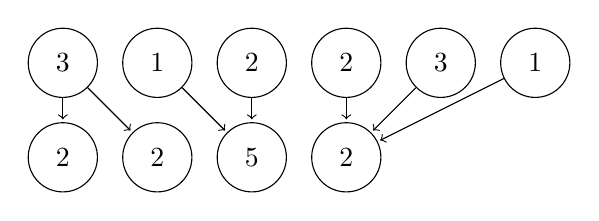
\begin{tikzpicture}[shorten >= 1pt, node distance = 1.2cm, on grid, auto] 
   \node[state] (q_0) {$3$};
   \node[state] (q_1) [right = of q_0] {$1$};
   \node[state] (q_2) [right = of q_1] {$2$};
   \node[state] (q_3) [right = of q_2] {$2$};
   \node[state] (q_4) [right = of q_3] {$3$};
   \node[state] (q_5) [right = of q_4] {$1$};
   \node[state] (q_6) [below = of q_0] {$2$};
   \node[state] (q_7) [right = of q_6] {$2$};
   \node[state] (q_8) [right = of q_7] {$5$};
   \node[state] (q_9) [right = of q_8] {$2$};
   \path[->]
    (q_0) edge node {} (q_6)
          edge node {} (q_7)
    (q_1) edge node {} (q_8)
    (q_2) edge node {} (q_8)
    (q_3) edge node {} (q_9)
    (q_4) edge node {} (q_9)
    (q_5) edge node {} (q_9);
\end{tikzpicture}
\end{center}

Para esta elección voraz se presentan las siguientes condiciones que hay que tener en cuenta.
\begin{itemize}
    \item Si los dos vectores de entrada ($A$ y $B$) son iguales,
        \begin{itemize}
            \item Si el tamaño de los vectores es multiplo de $3$.
            \item Si el tamaño de los vectores es multiplo de $3+1$.
            \item Si el tamaño de los vectores es multiplo de $3+2$.
        \end{itemize}
    \item Si las dos cadenas de entrada ($A$ y $B$) son diferentes.
\end{itemize}

Cuando se tiene dos vectores cuyo tamaño son múltiplos de 3, se puede hacer divisiones y agrupamientos de bloques de manera intercalada sin ningún problema. De esta manera, siempre se va a obtener \textit{i-divisiones} de la forma $(i,j_1),(i,j_2)$ y \textit{j-agrupamientos} de la forma $(i_1,j),(i_2,j)$, como se muestra a continuación.\\
\begin{center}
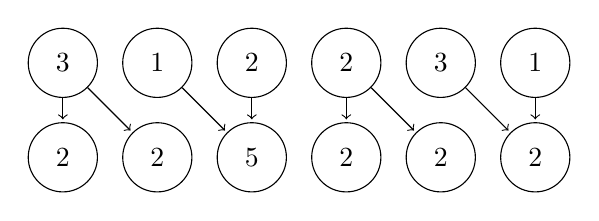
\begin{tikzpicture}[shorten >= 1pt, node distance = 1.2cm, on grid, auto] 
   \node[state] (q_0) {$3$};
   \node[state] (q_1) [right = of q_0] {$1$};
   \node[state] (q_2) [right = of q_1] {$2$};
   \node[state] (q_3) [right = of q_2] {$2$};
   \node[state] (q_4) [right = of q_3] {$3$};
   \node[state] (q_5) [right = of q_4] {$1$};
   \node[state] (q_6) [below = of q_0] {$2$};
   \node[state] (q_7) [right = of q_6] {$2$};
   \node[state] (q_8) [right = of q_7] {$5$};
   \node[state] (q_9) [right = of q_8] {$2$};
   \node[state] (q_10) [right = of q_9] {$2$};
   \node[state] (q_11) [right = of q_10] {$2$};
   \path[->]
    (q_0) edge node {} (q_6)
          edge node {} (q_7)
    (q_1) edge node {} (q_8)
    (q_2) edge node {} (q_8)
    (q_3) edge node {} (q_9)
          edge node {} (q_10)
    (q_4) edge node {} (q_11)
    (q_5) edge node {} (q_11);
\end{tikzpicture}
\end{center}
\verb| |\\
Para el caso cuando el tamaño de los vectores es un múltiplo de $3$ más $1$, al comienzo, se realizan las divisiones y agrupaciones de la misma manera, hasta que queden $4$ elementos por asignar. En este punto, se hace una división entre el primer elemento de $A$ que aún no ha sido asignado con todos los elementos sin asignar de $B$, menos el último. Luego, se hace una agrupación entre los elementos restantes de $A$ con el último elemento de $B$. Esta forma de match se muestra a continuación.\\
\begin{center}
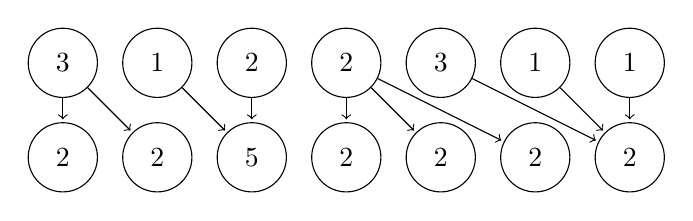
\begin{tikzpicture}[shorten >= 1pt, node distance = 1.2cm, on grid, auto] 
   \node[state] (q_0) {$3$};
   \node[state] (q_1) [right = of q_0] {$1$};
   \node[state] (q_2) [right = of q_1] {$2$};
   \node[state] (q_3) [right = of q_2] {$2$};
   \node[state] (q_4) [right = of q_3] {$3$};
   \node[state] (q_5) [right = of q_4] {$1$};
   \node[state] (q_6) [right = of q_5] {$1$};
   \node[state] (q_7) [below = of q_0] {$2$};
   \node[state] (q_8) [right = of q_7] {$2$};
   \node[state] (q_9) [right = of q_8] {$5$};
   \node[state] (q_10) [right = of q_9] {$2$};
   \node[state] (q_11) [right = of q_10] {$2$};
   \node[state] (q_12) [right = of q_11] {$2$};
   \node[state] (q_13) [right = of q_12] {$2$};
   \path[->]
    (q_0) edge node {} (q_7)
          edge node {} (q_8)
    (q_1) edge node {} (q_9)
    (q_2) edge node {} (q_9)
    (q_3) edge node {} (q_10)
          edge node {} (q_11)
          edge node {} (q_12)
    (q_4) edge node {} (q_13)
    (q_5) edge node {} (q_13)
    (q_6) edge node {} (q_13);
\end{tikzpicture}
\end{center}
\verb| |\\
Por último, para el caso cuando el tamaño de los vectores es un múltiplo de $3$ más $2$, al comienzo, se realizan las divisiones y agrupaciones de la misma manera que el caso 1, hasta que queden $5$ elementos por asignar. En este punto, se hace una división entre el primer elemento de $A$ que aún no ha sido asignado con todos los elementos sin asignar de $B$, menos el último. Luego, se hace una agrupación entre los elementos restantes de $A$ con el último elemento de $B$. Esta forma de match se muestra a continuación.\\
\begin{center}
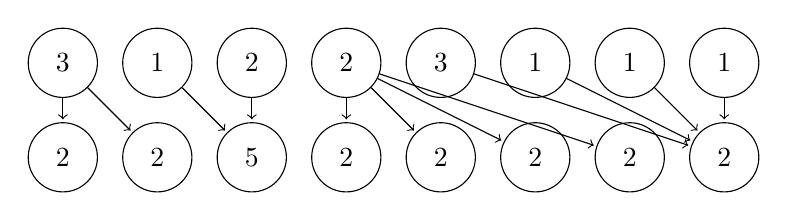
\begin{tikzpicture}[shorten >= 1pt, node distance = 1.2cm, on grid, auto] 
   \node[state] (q_0) {$3$};
   \node[state] (q_1) [right = of q_0] {$1$};
   \node[state] (q_2) [right = of q_1] {$2$};
   \node[state] (q_3) [right = of q_2] {$2$};
   \node[state] (q_4) [right = of q_3] {$3$};
   \node[state] (q_5) [right = of q_4] {$1$};
   \node[state] (q_6) [right = of q_5] {$1$};
   \node[state] (q_7) [right = of q_6] {$1$};
   \node[state] (q_8) [below = of q_0] {$2$};
   \node[state] (q_9) [right = of q_8] {$2$};
   \node[state] (q_10) [right = of q_9] {$5$};
   \node[state] (q_11) [right = of q_10] {$2$};
   \node[state] (q_12) [right = of q_11] {$2$};
   \node[state] (q_13) [right = of q_12] {$2$};
   \node[state] (q_14) [right = of q_13] {$2$};
   \node[state] (q_15) [right = of q_14] {$2$};
   \path[->]
    (q_0) edge node {} (q_8)
          edge node {} (q_9)
    (q_1) edge node {} (q_10)
    (q_2) edge node {} (q_10)
    (q_3) edge node {} (q_11)
          edge node {} (q_12)
          edge node {} (q_13)
          edge node {} (q_14)
    (q_4) edge node {} (q_15)
    (q_5) edge node {} (q_15)
    (q_6) edge node {} (q_15)
    (q_7) edge node {} (q_15);
\end{tikzpicture}
\end{center}
\verb||\\
Ahora, para los casos en los que los vectores tienen diferentes tamaños, se debe hacer una división de ambos vectores hasta que tengan el tamaño del vector menor menos $1$. Así, tendríamos dos vectores del mismo tamaño que se puede procesar con cualquiera de las maneras ya mencionadas. Y para los nodos restantes, quedarían hacer una divisón si es que el tamaño original del vector $A$ es menor que el tamaño original de $B$, y un agrupamiento en caso contrario, como se muestra a continuación.\\
\begin{center}
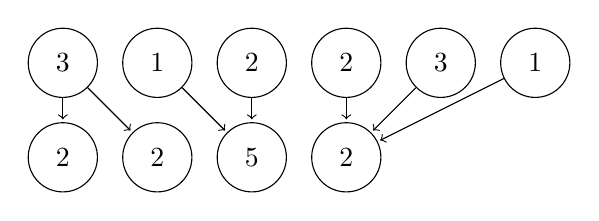
\begin{tikzpicture}[shorten >= 1pt, node distance = 1.2cm, on grid, auto] 
   \node[state] (q_0) {$3$};
   \node[state] (q_1) [right = of q_0] {$1$};
   \node[state] (q_2) [right = of q_1] {$2$};
   \node[state] (q_3) [right = of q_2] {$2$};
   \node[state] (q_4) [right = of q_3] {$3$};
   \node[state] (q_5) [right = of q_4] {$1$};
   \node[state] (q_6) [below = of q_0] {$2$};
   \node[state] (q_7) [right = of q_6] {$2$};
   \node[state] (q_8) [right = of q_7] {$5$};
   \node[state] (q_9) [right = of q_8] {$2$};
   \path[->]
    (q_0) edge node {} (q_6)
          edge node {} (q_7)
    (q_1) edge node {} (q_8)
    (q_2) edge node {} (q_8)
    (q_3) edge node {} (q_9)
    (q_4) edge node {} (q_9)
    (q_5) edge node {} (q_9);
\end{tikzpicture}
\end{center}

El pseudocódigo de este algoritmo voraz para el problema se muestra en el algoritmo 2 \textsc{Min-Matching-Voraz}.

\begin{algorithm}
\caption{\textsc{Min-Matching-Voraz}}
\algsetup{linenosize=\small}
\scriptsize
\begin{algorithmic}
\REQUIRE Dos arreglos $A$ y $B$ con la suma de unos por bloque.
\ENSURE Un matching entre $A$ y $B$, y su peso.
\begin{flushleft}
\textsc{Min-Matching-Voraz}$(A,B)$
\end{flushleft}
    \STATE $result=\emptyset$
    \IF{$A.length=B.length$}
        \IF{$A.length$ $mod$ $3=0$}
            \STATE $result=$ \textsc{Match-Mult-3}$(A,B)$
        \ELSIF{$A.length$ $mod$ $3=1$}
            \STATE $result=$ \textsc{Match-Mult-3-1}$(A,B)$
        \ELSE
            \STATE $result=$ \textsc{Match-Mult-3-2}$(A,B)$
        \ENDIF
    \ELSE
        \IF{$A.length>B.length$}
            \STATE $A'=A[1:B.length-1]$
            \STATE $B'=B[1:B.length-1]$
            \IF{$A'.length$ $mod$ $3=0$}
                \STATE $result=$ \textsc{Match-Mult-3}$(A',B')$
            \ELSIF{$A'.length$ $mod$ $3=1$}
                \STATE $result=$ \textsc{Match-Mult-3-1}$(A',B')$
            \ELSE
                \STATE $result=$ \textsc{Match-Mult-3-2}$(A',B')$
            \ENDIF
            \STATE $t=A[B.length:A.length]$
            \STATE $result.add(t,B[B.length])$
        \ELSE
            \STATE $A'=A[1:A.length-1]$
            \STATE $B'=B[1:A.length-1]$
            \IF{$A'.length$ $mod$ $3=0$}
                \STATE $result=$ \textsc{Match-Mult-3}$(A',B')$
            \ELSIF{$A'.length$ $mod$ $3=1$}
                \STATE $result=$ \textsc{Match-Mult-3-1}$(A',B')$
            \ELSE
                \STATE $result=$ \textsc{Match-Mult-3-2}$(A',B')$
            \ENDIF
            \STATE $t=A[A.length:B.length]$
            \STATE $result.add(A[A.length],t)$
        \ENDIF
    \ENDIF
    \RETURN $result$
\end{algorithmic}
\label{alg:min-matching-voraz}
\end{algorithm}

\section{Pregunta 2: Recurrencia}
Tenemos la siguiente recurrencia para el problema de \textsc{Min-Matching}.
\begin{center}
\[ OPT(i,j) =
   \begin{cases}
     \frac{A_i}{\sum _{k=1}^iB_k} & \text{para todo $i=1$} \\
     \frac{\sum _{k=1}^iA_k}{B_j} & \text{para todo $j=1$} \\
     min(min_{l=1}^{j-1}\{OPT(i-1, & \text{otro caso} \\
     j-l)+\frac{A_i}{\sum _{k=j-l+1}^jB_k}\}; & \\
     min_{l=1}^{i-1}\{OPT(i-l,j-1) & \\
     +\frac{\sum _{k=i-l+1}^iA_k}{B_j}\}) &
   \end{cases}
\]
\end{center}
\section{Pregunta 3: Recursivo}
\subsection{Recurrencia de complejidad}
Tenemos la siguiente recurrencia de complejidad para el problema de \textsc{Min-Matching-Recursivo}.\\
\begin{center}
\[ C(m,n) =
   \begin{cases}
     2*c_1 & \text{para todo $i=2$ \text{ó} $j=2$} \\\\
     \sum _{n=1}^{n-1}C\left(m-1,n-h\right)+ & \text{otro caso} \\
     \sum _{n=1}^{m-1}C\left(m-h,n-1\right)+ & \\
     \Omega \left(1\right) & 
   \end{cases}
\]
\end{center}

\subsection{Demostración de complejidad}
Tenemos lo siguiente:\\\\
$C\left(m;n\right)=\sum _{n=1}^{n-1}C\left(m-1;n-h\right)+$\\\\
$\sum _{n=1}^{m-1}C\left(m-h;n-1\right)+\Omega \left(1\right)\ge C\left(m-1;n-1\right)+$\\\\
$C\left(m-1;n-1\right)$\\

$\therefore C\left(m;n\right)\ge C\left(m-1;n-1\right)+C\left(m-1;n-1\right)$

\[
 \boxed{C\left(m;n\right)\ge 2C\left(m-1;n-1\right)}
 \]

\textit{Hipótesis}: $C\left(m;n\right)=\Omega \left(2^r\right)$, $r$ es máximo\\
$\Rightarrow \:C\left(m;n\right)\ge \:C\cdot \:2^r\:\leftrightarrow \:m\:\wedge \:n\:\ne \:1$\\\\

\textit{Adicional}:
$C\left(2;2\right)=2\cdot K\ge 2^2\cdot C$\\
$k=2\:\wedge \:C=1$\\

\begin{align*}
   C\left(2;2\right)&=\Omega \left(2^2\right) \\
   &\vdots\\
   C\left(m-1;n-1\right)&=\Omega \left(2^{r-1}\right)\\
   C\left(m;n\right)&=\Omega \left(2^r\right)
\end{align*}

Por hipótesis inductiva, tenemos:\\\\
$C\left(m;n\right)\ge 2\cdot C\left(m-1;n-1\right)$\\\\
$2^r\cdot K\ge 2\cdot 2^{r-1}\cdot K_1$\\\\
$K\cdot \:2\:\wedge \:K_1=1$ \textbf{Se verifica}\\\\
$C\left(m;n\right)=\Omega \:\left(2^{max\left\{m,n\right\}}\right);\:m\:\wedge \:n \neq 1$

\subsection{Algoritmo recursivo}
Para resolver el problema de \textsc{Min-Matching} se ha planteado el siguiente pseudocódigo.
\begin{algorithm}
\caption{\textsc{Min-Matching-Recursivo}}
\algsetup{linenosize=\small}
\scriptsize
\begin{algorithmic}
\REQUIRE Dos arreglos $A$ y $B$ con la suma de unos por bloque.
\ENSURE Un matching entre $A$ y $B$, y su peso.
\begin{flushleft}
\textsc{Min-Matching-Recursivo}$(A,B)$
\end{flushleft}
    \STATE $i=A.length$
    \STATE $j=B.length$
    \IF{$i=1$ \AND $j=1$}
        \RETURN $\{(A[i],B[j])\}$
    \ELSIF{$i=1$ \OR $j=1$}
        \IF{$i=1$}
            \STATE $match=(A[i],\emptyset)$
            \FOR{$a=1$ to $j+1$}
                \STATE $match[2].add(B[a])$
            \ENDFOR
            \RETURN $\{match\}$
        \ELSE
            \STATE $match=(\emptyset,B[j])$
            \FOR{$a=1$ to $i+1$}
                \STATE $match[1].add(A[a])$
            \ENDFOR
            \RETURN $\{match\}$
        \ENDIF
    \ELSE
        \STATE $pesos=\emptyset$
        \STATE $match=$ \textsc{Min-Matching-Recursivo}$(A[1:i],B[1:j])$
        \STATE $match.add(A[i],B[j])$
        \STATE $pesos.add(match)$
        \FOR{$a=1$ to $i$}
            \STATE $matches=$ \textsc{Min-Matching-Recursivo}$(A[1:a],B[1:j])$
            \STATE $match=(\emptyset,B[j])$
            \FOR{$b=a$ to $i+1$}
                \STATE $match[1].add(A[b])$
            \ENDFOR
            \STATE $matches.add(match)$
            \STATE $pesos.add(matches)$
        \ENDFOR
        \FOR{$a=2$ to $j$}
            \STATE $matches=$ \textsc{Min-Matching-Recursivo}$(A[1:i],B[1:a])$
            \STATE $match=(A[i],\emptyset)$
            \FOR{$b=a$ to $j+1$}
                \STATE $match[2].add(B[b])$
            \ENDFOR
            \STATE $matches.add(match)$
            \STATE $pesos.add(matches)$
        \ENDFOR
    \RETURN $min(pesos)$
    \ENDIF
\end{algorithmic}
\label{alg:min-matching-recursivo}
\end{algorithm}
\verb| |\\
\section{Pregunta 4: Memorizado}

\subsection{Arbol de análisis de costo}

\begin{center}
    \begin{forest}
for tree={l sep-=.2em,l=0},
[\scalebox{0.6}{
$\begin{array}{c}
M(m,n)
\end{array}$}
 [\scalebox{0.6}{
$\begin{array}{c}
min(m-1,n'-1)
\end{array}$}
  [\scalebox{0.6}{
$\begin{array}{c}
M(m-1,1) \text{...}
\end{array}$}
  ]
  [\scalebox{0.6}{
$\begin{array}{c}
\text{...} M(m-1,n-1)
\end{array}$}
  ]
 ]
 [\scalebox{0.6}{
$\begin{array}{c}
min(m'-1,n-1)
\end{array}$}
  [\scalebox{0.6}{
$\begin{array}{c}
M(1,n-1) \text{...}
\end{array}$}
  ]
  [\scalebox{0.6}{
$\begin{array}{c}
\text{...} M(m-1,n-1)
\end{array}$}
  ]
 ]
]
\end{forest}
\end{center}
\begin{align*}
   &\vdots
\end{align*}
\begin{FlushRight}
    \begin{forest}
for tree={l sep-=.2em,l=0},
[\scalebox{0.6}{
$\begin{array}{c}
M(m-(n-1),1)
\end{array}$}
 [\scalebox{0.6}{
$\begin{array}{c}
M(1,1) \text{...}
\end{array}$}
 ]
 [\scalebox{0.6}{
$\begin{array}{c}
\text{...} M(m-n+1,1)
\end{array}$}
 ]
]
\end{forest}
\end{FlushRight}

\subsection{Recurrencia de complejidad}
Tenemos la siguiente recurrencia para el problema de \textsc{Min-Matching-Memorizado}.\\
\begin{center}
\[ C(m,n) =
   \begin{cases}
     c_1*n & \text{para todo $i=1$} \\
     c_1*m & \text{para todo $j=1$} \\
     C(m-1,n-1)+k(n-2)+d & \text{otro caso}
   \end{cases}
\]
\end{center}

\subsection{Demostración de complejidad}
\text{Suponiendo que} $m>n$ :\\ \\
\begin{math}
    C(m,n) = C(m-1,n-1) + k(m-2)+ d\\
    =C(m-2,n-2)+k(m-2)+k(m-3)+2d\\
    =C(m-2,n-2)+2km-k(2+3)+2d\\
    =C(m-3,n-3)+3km-k(2+3+4)+3d\\
    \vdots\\
    =C(m-(n-1),n-(n-1))+ (n-1)km-\\ k(2+3+4...+n)+(n-1)d\\
    =C(m-(n-1),1)+(n-1)km-k(\frac{n*(n+1)}{2}-1)+(n-1)d\\
    =O(m)+(n-1)km+O(n^2)+O(n) 
\end{math}\\ \\
\text{Se verifica que }$O(m)$, $O(n)$ y $O(n^2)$ son $O(m*n)$\\
\text{Entonces: }\\
Faltaría demostrar que $(n-1)km = O(m*n)$\\ 
\begin{math}
    k*nm-k*m \leq c*mn\\
    k-\frac{k}{n} \leq c \\
    \text{Con c = 1 }n_0\text{=1; } n \geq n_0 >0\\
    0 \leq c \\
    \Rightarrow (n-1)km = O(n*m) \\ \\
    \textbf{Conluimos: } 
    C(m,n) = O(n*m)
\end{math}

\begin{algorithm}
\caption{\textsc{Min-Matching-Memoizado}}
\algsetup{linenosize=\small}
\scriptsize
\begin{algorithmic}
\REQUIRE Dos arreglos $A$ y $B$ con la suma de unos por bloque.
\ENSURE Un matching entre $A$ y $B$, y su peso.
\begin{flushleft}
\textsc{Min-Matching-Memoizado}$(A,B)$
\end{flushleft}
    \STATE $i=A.length$
    \STATE $j=B.length$
    \IF{$i=1$ \AND $j=1$}
        \RETURN $\{(A[i],B[j])\}$
    \ELSIF{$i=1$ \OR $j=1$}
        \IF{$i=1$}
            \STATE $match=(A[i],\emptyset)$
            \FOR{$a=1$ to $j+1$}
                \STATE $match[2].add(B[a])$
            \ENDFOR
            \RETURN $\{match\}$
        \ELSE
            \STATE $match=(\emptyset,B[j])$
            \FOR{$a=1$ to $i+1$}
                \STATE $match[1].add(A[a])$
            \ENDFOR
            \RETURN $\{match\}$
        \ENDIF
    \ELSE
        \IF{$memoria.get(i)$}
            \IF{$memoria[i].get(j)$}
                \RETURN $memoria[i][j]$
            \ENDIF
        \ENDIF
        \STATE $pesos=\emptyset$
        \STATE $match=$ \textsc{Min-Matching-Memorizado}$(A[1:i],B[1:j])$
        \STATE $match.add(A[i],B[j])$
        \STATE $pesos.add(match)$
        \FOR{$a=2$ to $i$}
            \STATE $matches=$ \textsc{Min-Matching-Memorizado}$(A[1:a],B[1:j])$
            \STATE $match=(\emptyset,B[j])$
            \FOR{$b=a$ to $i+1$}
                \STATE $match[1].add(A[b])$
            \ENDFOR
            \STATE $matches.add(match)$
            \STATE $pesos.add(matches)$
        \ENDFOR
        \FOR{$a=2$ to $j$}
            \STATE $matches=$ \textsc{Min-Matching-Memorizado}$(A[1:i],B[1:a])$
            \STATE $match=(A[i],\emptyset)$
            \FOR{$b=a$ to $j+1$}
                \STATE $match[2].add(B[b])$
            \ENDFOR
            \STATE $matches.add(match)$
            \STATE $pesos.add(matches)$
        \ENDFOR
        \STATE $minp = min(pesos)$
        \IF{$memoria.get(i)$}
            \STATE $memoria[i][j] = minp$
        \ELSE
            \STATE $memoria[i] = dic()$
            \STATE $memoria[i][j] = minp$
        \ENDIF
        \RETURN $memoria[i][j]$
    \ENDIF
\end{algorithmic}
\label{alg:min-matching-memoizado}
\end{algorithm}
\verb||\\
\section{Pregunta 5: Programación Dinámica}
El algoritmo en Programación Dinámica esta basado en el Memorizado principalmente, al ser este muy largo optamos por no colocarlo aquí, sin embargo se puede visualizar en el \href{https://github.com/Piero16301/Proyecto_ADA/blob/master/Source/functionsVectors/matchDP.py}{\textbf{siguiente enlace}}. En este algoritmo se utilizan variables que actúan tanto como stacks como contadores, entre estas están:
\begin{itemize}
    \item \textbf{min}: Aquí se almacena el match mínimo, este va actualizándose conforme se vayan descubriendo nuevos matches
    \item \textbf{mem}: Aquí se almacena la matriz de memoria, esta crece conforme se van descubriendo nuevos matches
    \item \textbf{actual}: Esta variable actúa como stack en donde se van formando los distintos matches, cuando esta completo, si es que su valor total es menor que el mínimo actual, esta se vuelve el mínimo actual
    \item \textbf{counters}: Aquí almacenamos un stack de contadores que se encarga de actualizar en tiempo real las combinaciones de configuraciones posibles dentro de un match
    \item \textbf{possible\_values}: Aquí almacenamos un stack que va sincronizado con counters y que se encarga de ir guardando los matches que sirven para buscar el mínimo en su nivel que a su vez ayuden a formar la memoria
    \item \textbf{i, j}: Aquí se almacenan las posiciones en el primer y segundo vector
\end{itemize}% YAY :D

\section{Transformación de imágenes}
Dadas dos matrices $A[1...p, 1...q]$, $B[1...p,1...q]$ de ceros y unos, una \textit{transformación} de $A$ en $B$ es un conjunto $M=\{M_1,M_2,...,M_p\}$, donde cada $M_i$ es un matching entre los vectores $A[i]$ y $B[i]$. El peso de $M$, denotado por $w(M)$ es igual a la suma de pesos de cada $M_i$ es decir, de acuerdo a lo siguiente.

$$w(M)=\sum _{i=1}^nw\left(M_i\right)$$

\subsection{Problema Min-Transformacion}
Dadas dos matrices $A$ y $B$ de ceros y unos, encontrar una transformación entre $A$ y $B$ de peso mínimo.

Es claro que para resolver el problema \textsc{Min-Transformacion} de manera óptima basta invocar varias veces a alguna de las subrutinas implementadas en la sección anterior.

\section{Pregunta 6: Transformación Voráz}
Analise, diseñe e implemente un algoritmo voráz con complejidad cuadrática para el problema \textsc{Min-Transformacion}. Su algoritmo no deberá encontrar necesariamente la transformación de peso mínimo. Debe usar como subrutina al algoritmo implementado en la Pregunta 1.\\\\
\textit{Entrada del algoritmo}: Dos matrices $A$ y $B$ de ceros y unos de tamaño $p \times q$.\\\\
\textit{Salida del algoritmo}: Una transformación entre $A$ y $B$, no necesariamente óptima, y su peso.\\\\
\textit{Tiempo de ejecución del algoritmo}: $O(pq)$\\\\
Para el planteamiento de la solución voráz a este problema, primero se ha realizado una llamada iterativa al Algoritmo \ref{alg:vector-converter} para realizar la conversión de una matriz de unos y ceros a una matriz de pesos de los bloques (números enteros). Entonces, a partir de esto se puede construir este nuevo algoritmo.

\begin{algorithm}
\caption{\textsc{Matrix-Converter}}
\algsetup{linenosize=\small}
\scriptsize
\begin{algorithmic}
\REQUIRE Una matriz $A$ de unos y ceros.
\ENSURE Una matriz $A'$ con la suma de unos para cada bloque.
\begin{flushleft}
\textsc{Matrix-Converter}$(A)$
\end{flushleft}
    \STATE $resultado=\emptyset$
    \FOR{$row$ in  $A$}
        \STATE $resultado=resultado \cup \textsc{Vector-Converter}(row)$
    \ENDFOR
    \RETURN $resultado$
\end{algorithmic}
\label{alg:matrix-converter}
\end{algorithm}
\verb||\\
Ahora, se ha planteado como solución para el problema de \textit{Min-Transformación} llamar de forma iterativa al Algoritmo \ref{alg:min-matching-voraz} para cada fila de las matrices. Como dice el planteamiento del problema, se debe de hacer un \textsc{Match} entre las filas de ambas matrices, y el índice de la fila sea el mismo en ambas. A partir de esto, se ha planteado el siguiente algoritmo.

\begin{algorithm}
\caption{\textsc{Min-Transformacion-Voraz}}
\algsetup{linenosize=\small}
\scriptsize
\begin{algorithmic}
\REQUIRE Dos matrices $A$ y $B$ con la suma de unos por bloque.
\ENSURE Una transformación entre $A$ y $B$, y su peso.
\begin{flushleft}
\textsc{Min-Transformacion-Voraz}$(A,B)$
\end{flushleft}
    \STATE $resultado=\emptyset$
    \STATE $peso=0$
    \FOR{$i=0$ to $A.rows$}
        \STATE $resultado=resultado$ $\cup$ $\textsc{Min-Matching-Voraz}(A[i],B[i])$
    \ENDFOR
    \FOR{$i=0$ to $resultado.size$}
        \STATE $peso=peso+\textsc{Sum}(resultado[i])$
    \ENDFOR
    \RETURN $[resultado,peso]$
\end{algorithmic}
\label{alg:min-transformacion-voraz}
\end{algorithm}
\verb||\\
Para poder calcular la suma de los \textit{match} de cada fila, se ha creado una función, la cual se muestra a continuación.

\begin{algorithm}
\caption{\textsc{Sum}}
\algsetup{linenosize=\small}
\scriptsize
\begin{algorithmic}
\REQUIRE Un \textit{match} entre dos arreglos.
\ENSURE El peso del \textit{match} inicial.
\begin{flushleft}
\textsc{Sum}$(match)$
\end{flushleft}
    \IF{$match.length=0$}
        \RETURN $0$
    \ENDIF
    \STATE $resultado=0$
    \FOR{$i$ in $match$}
        \STATE $resultado=resultado+peso(i)$
    \ENDFOR
    \RETURN $resultado$
\end{algorithmic}
\label{alg:sum}
\end{algorithm}

\section{Pregunta 7: Transformación Prog. Dinámica}
Para la transformacion de Programacion Dinamica se aplico la misma estrategis vista previamente simplemente reemplazando la funcion que haya los matchings.

\begin{algorithm}
\caption{\textsc{Min-Transformacion-Dinamico}}
\algsetup{linenosize=\small}
\scriptsize
\begin{algorithmic}
\REQUIRE Dos matrices $A$ y $B$ con la suma de unos por bloque.
\ENSURE Una transformación entre $A$ y $B$, y su peso.
\begin{flushleft}
\textsc{Min-Transformacion-Dinamico}$(A,B)$
\end{flushleft}
    \STATE $resultado=\emptyset$
    \STATE $peso=0$
    \FOR{$i=0$ to $A.rows$}
        \STATE $resultado=resultado$ $\cup$ $\textsc{Min-Matching-Dinamico}(A[i],B[i])$
    \ENDFOR
    \FOR{$i=0$ to $resultado.size$}
        \STATE $peso=peso+\textsc{Sum}(resultado[i])$
    \ENDFOR
    \RETURN $[resultado,peso]$
\end{algorithmic}
\label{alg:min-transformacion-dinamico}
\end{algorithm}

\section{Pregunta 8: Lectura de Imágenes}
La motivación de hacer transformación de una matriz hacia otra es poder transformar
una imagen en otra mediante una curva suave. Una manera de hacerlo es codificar cada pixel como un 0 o un 1. Para ello, puede tomar cada pixel en la escala RGB (r, g, b) y transformarlo a una escala de grises, para posteriormente escoger los que están más cerca de ser pixeles blancos (0) y los que están más cerca de ser negros (1). Existen muchos métodos para hacer esta transformación, dependiendo de los coeficientes escogidos.\\

Las fórmulas correspondientes para realizar esta conversión, puede ser con Rec. 601 Luma, la cual puede ser calculada con cualquiera de las siguientes fórmulas.

\begin{equation}
    Y'_{601}=0.299R'+0.587G'+0.114B'
\end{equation}

\begin{equation}
    Y'_{709}=0.2126R'+0.7152G'+0.0722B'
\end{equation}

\begin{equation}
    Y'_{240}=0.212R'+0.701G'+0.087B'
\end{equation}

Aplicando estas fórmulas, se consigue construir una matriz nueva en escala de grises. Es decir, se ha realizado una transformación de $R^3$ a $R^2$. El proceso de transformación de esta matriz, sigue la siguiente forma.

\begin{figure}[H]
  \centering
  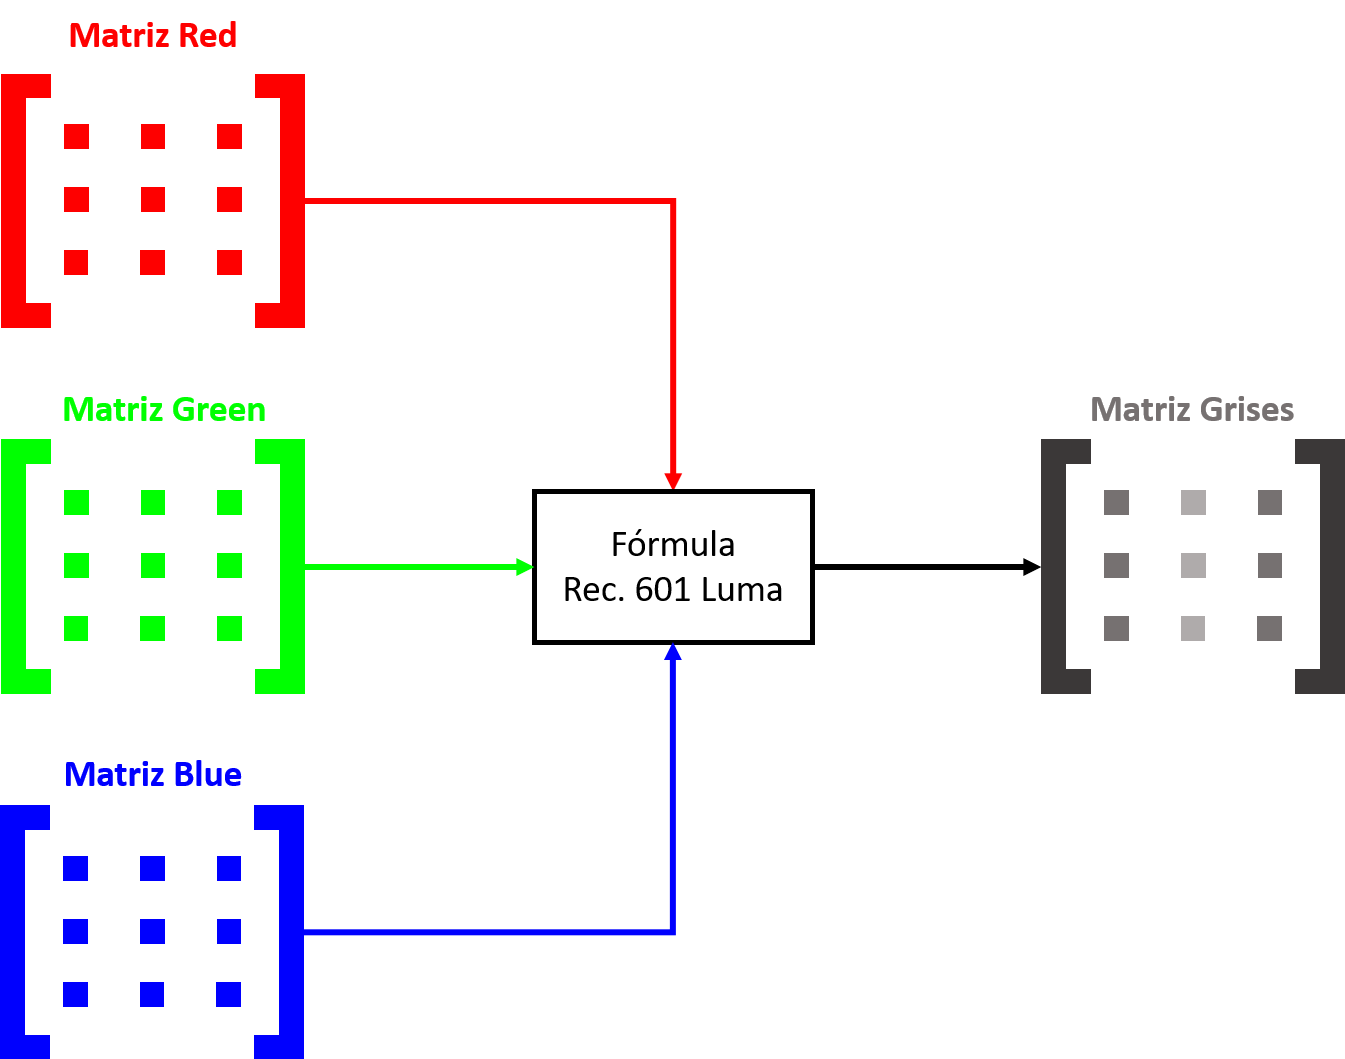
\includegraphics[scale=0.35]{images/matriz_grises.png}
  \caption[Grises]{Transformación de matrices RGB en matriz de escala de grises}
  \label{fig:grises}
\end{figure}

Finalmente, para convertirlo a una matriz de unos y ceros, se define un umbral, para que se defina para cada casilla de la matriz de escala de grises, si esta se va a convertir en 1 o 0, como se muestra a continuación.

\begin{figure}[H]
  \centering
  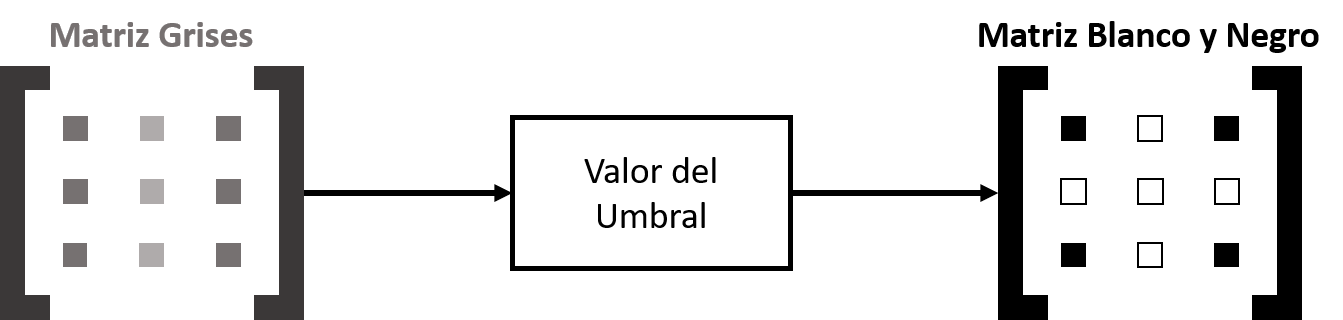
\includegraphics[scale=0.35]{images/matriz_negro.png}
  \caption[Negro]{Transformación de matriz de escala de grises en matriz de 1's y 0's}
  \label{fig:negro}
\end{figure}

\section{Pregunta 9: Animación}
Se va a implementar una animación que va a mostrar el proceso de transformación de una imagen en otra usando los algoritmos de transformación \textsc{Voráz}, \textsc{
Prog. Dinámica} y \textsc{Prog. Dinámica Mejorada}.
\verb||\\\\
Para construir la animación, va a ser necesario crear imágenes intermedias que van a mostrar un pequeño cambio cuando se va a ir pasando de una en una. De esta manera, cuando se reproduzcan de manera rápida, se va a poder visualizar en forma de animación. Para la construcción de estas imágenes intermedias, se van a tener en cuenta los siguientes casos.

\subsection{Agrupación}
Cuando se tiene una agrupación en una transformación, lo que se tiene que hacer es calcular la cantidad de píxeles que se van a ir moviendo por cada imagen intermedia.
\verb||\\\\
Para este caso, se debe realizar el cálculo de cuantas imágenes intermedias se van a querer generar, así como también, el tamaño de los bloques de unos de ambas matrices para saber qué cantidad de píxeles se van a convertir en la imagen resultante. Este proceso se puede ver en la siguiente imagen.

\begin{figure}[H]
  \centering
  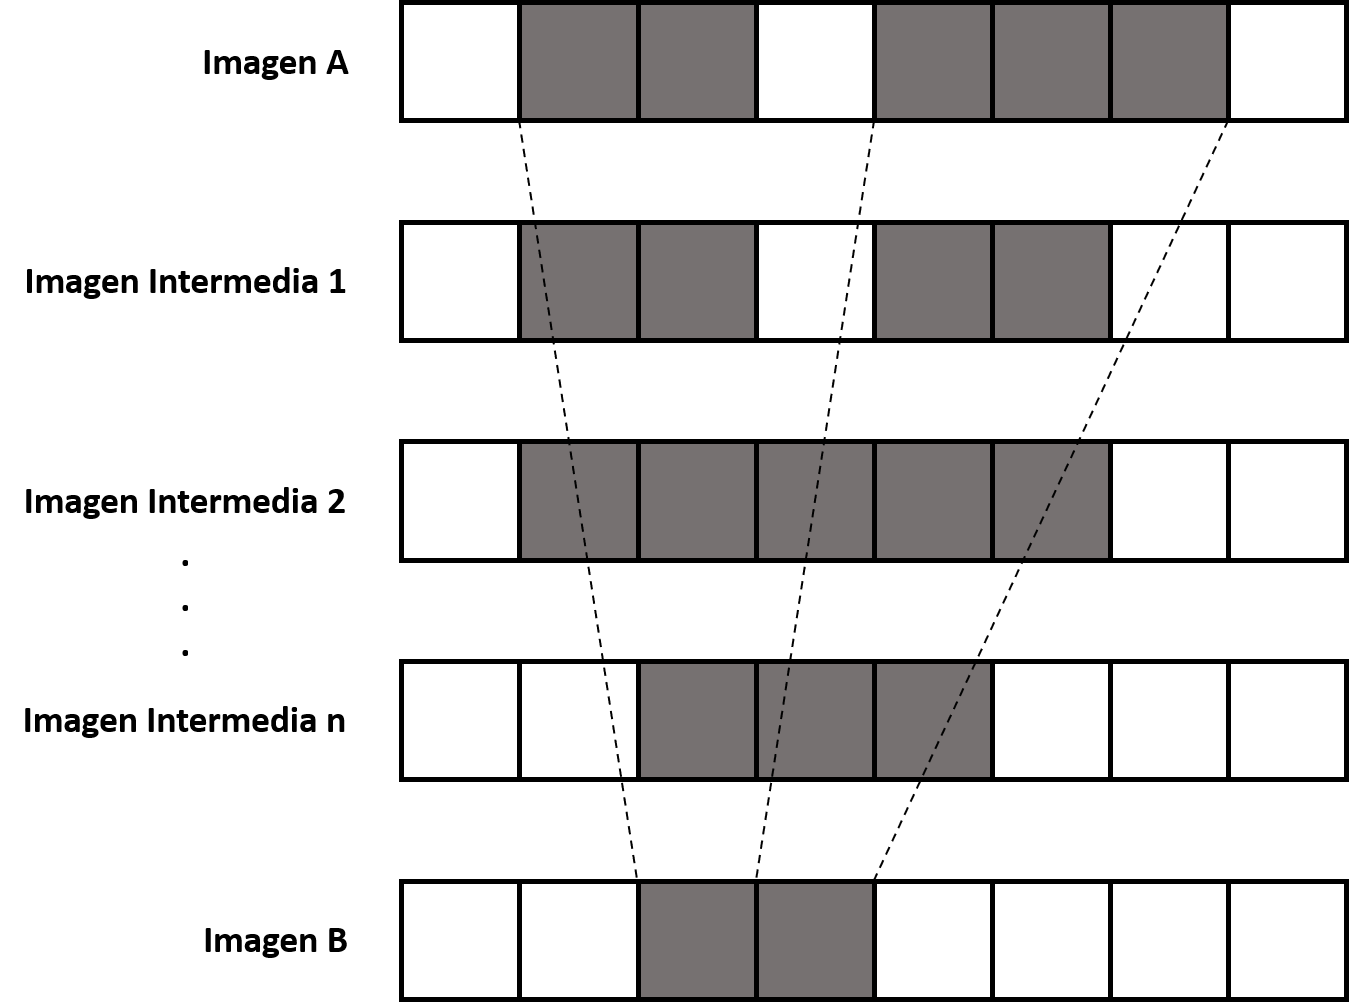
\includegraphics[scale=0.35]{images/agrupacion.png}
  \caption[agrupacion]{Creación de imágenes intermedias para una agrupación}
  \label{fig:agrupacion}
\end{figure}

\subsection{División}
Cuando se tiene una división en una transformación, lo que se tiene que hacer es calcular la cantidad de píxeles que se van a ir moviendo por cada imagen intermedia.
\verb||\\\\
Para este caso, se debe realizar el cálculo de cuantas imágenes intermedias se van a querer generar, así como también, el tamaño de los bloques de unos de ambas matrices para saber qué cantidad de píxeles se van a convertir en la imagen resultante. Este proceso se puede ver en la siguiente imagen.

\begin{figure}[H]
  \centering
  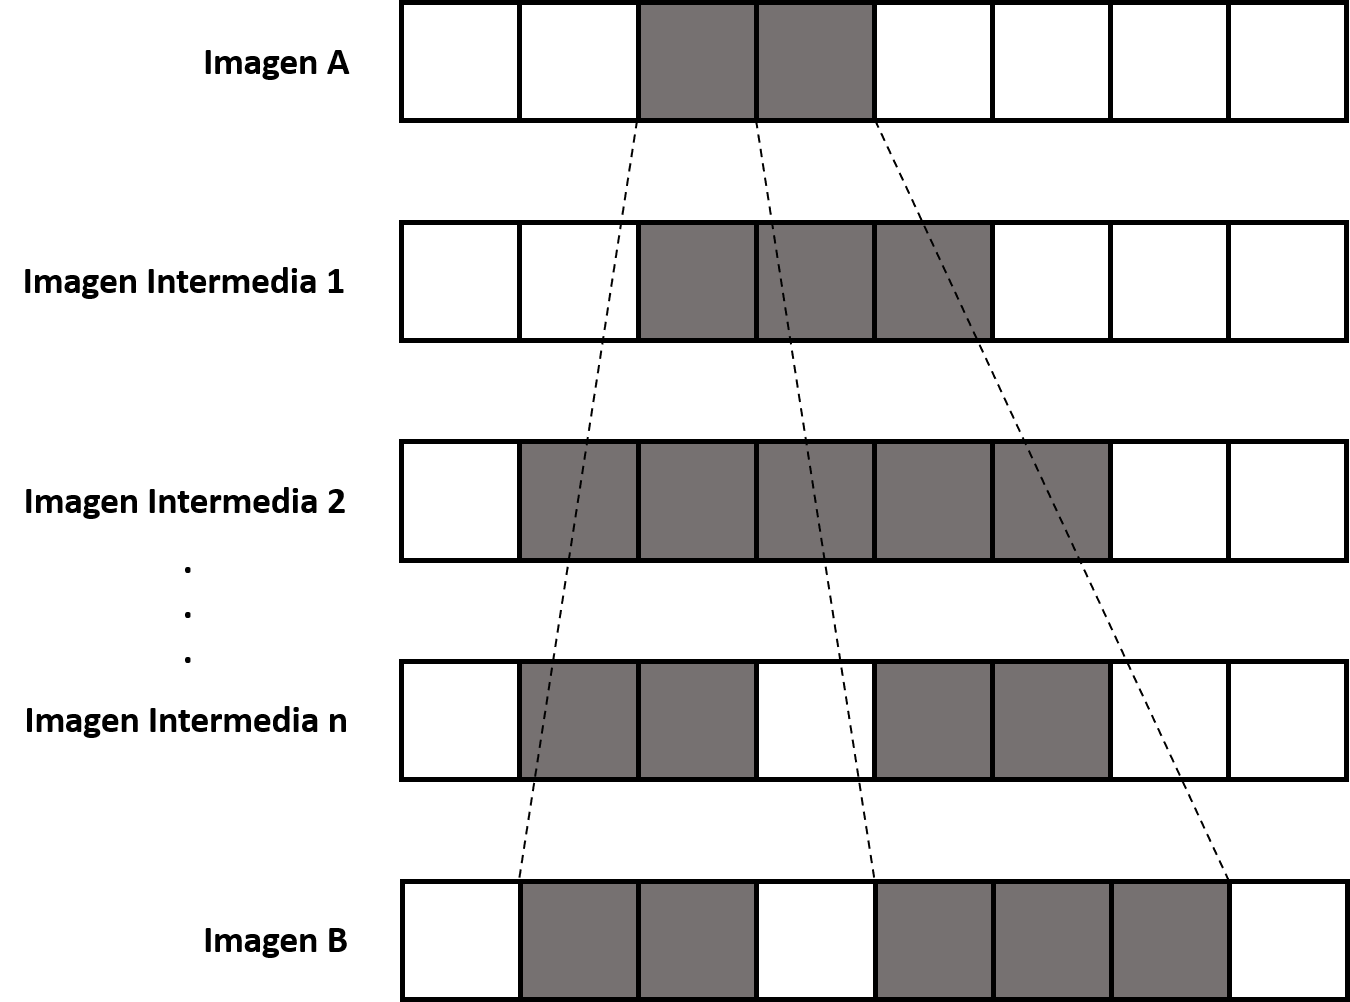
\includegraphics[scale=0.35]{images/division.png}
  \caption[division]{Creación de imágenes intermedias para una división}
  \label{fig:division}
\end{figure}

\section{Pregunta 10: Dinámica Mejorada}

\begin{algorithm}
\caption{\textsc{Min-Transformacion-Mejorado}}
\algsetup{linenosize=\small}
\scriptsize
\begin{algorithmic}
\REQUIRE Dos matrices $A$ y $B$ con la suma de unos por bloque.
\ENSURE Una transformación entre $A$ y $B$, y su peso.
\begin{flushleft}
\textsc{Min-Transformacion-Dinamico-Mejorado}$(A,B)$
\end{flushleft}
    \STATE $resultado=\emptyset$
    \STATE $peso=0$
    \FOR{$i=0$ to $A.rows$}
        \STATE $resultado=resultado$ $\cup$ $\textsc{Min-Matching-Mejorado}(A[i],B[i])$
    \ENDFOR
    \FOR{$i=0$ to $resultado.size$}
        \STATE $peso=peso+\textsc{Sum}(resultado[i])$
    \ENDFOR
    \RETURN $[resultado,peso]$
\end{algorithmic}
\label{alg:min-transformacion-dinamico-mejorado}
\end{algorithm}

La mayor diferencia respecto a el dinámico normal fue la variación de nuestra función de peso la cual ahora recibía también el valor $u$ como parámetro el cual se hallaria dentro de nuestra función dinámica mejorada
\begin{algorithm}
\caption{\textsc{Peso}}
\algsetup{linenosize=\small}
\scriptsize
\begin{algorithmic}
\REQUIRE Una configuración dentro de un match y el valor $u$
\ENSURE El valor de la configuracion de el match
\begin{flushleft}
\textsc{Peso}$(conf, u)$
\end{flushleft}
    \IF{isinstance($conf[0]$, int) \AND isinstance($conf[1]$, int)}
        \RETURN abs($conf[0]/conf[1] - u$)
    \ELSIF{isinstance($conf[0]$, int)}
        \STATE $temp$ = $conf[0]$
        \STATE $sum$ = $0$
        \FOR{i = 0 to len($conf[1]$)}
            \STATE $sum$ = $sum$ + $conf[1][i]$
        \ENDFOR
        \RETURN abs($temp/sum - u$)
    \ELSE
        \STATE $temp$ = $conf[1]$
        \STATE $sum$ = $0$
        \FOR{i = 0 to len($conf[0]$)}
            \STATE $sum$ = $sum$ + $conf[1][i]$
        \ENDFOR
        \RETURN abs($sum/temp - u$)
    \ENDIF
\end{algorithmic}
\label{alg:min-transformacion-peso}
\end{algorithm}

\renewcommand{\appendixname}{Anexos}
\renewcommand{\appendixtocname}{Anexos}
\renewcommand{\appendixpagename}{Anexos}

\appendix
\verb||\\
Link repositorio GitHub: \href{https://github.com/Piero16301/Proyecto_ADA.git}{\underline{Proyecto ADA}}

\end{document}